\documentclass[11pt]{article}
%Gummi|065|=)
\title{\textbf{CARACTERISTICAS DE LOS CONVERTIDORES DE POTENCIA CA-CD-CA,CD-CA,CA-CA Y CD-CD}}
\author{Mejorada Lopez Ivan\\
		sistemas electronicos de interfaz\\
	    4B	}
\date{14/09/19}
\usepackage{graphicx}
\usepackage[hidelinks]{hyperref}

\begin{document}

\maketitle
\begin{figure}[htp]
\centering

\includegraphics[scale=1.00]{UPZMG_Prueba_1b.png}
\caption{}
\label{}
\end{figure}




\section{¿Que son los convertidores de potencia}
8
Los convertidores son elementos capaces de alterar las caracteristicasde la tension y la corriente que reciben,tenasformandola de manera optimizada para los usos especificos donde va a ser destinada para cada caso.El espectacular avance de las telecomunicaciones en los ultimos años tambien ha contribuido en gran medida al aumento del numero de equipos electronicos conectados a la red de distribucion electrica de baja tension. Hay estudios que afirman que un 50 porciento de la energia electrica consumida hoy en dia los paises mas desarrollados sufren algun proceso electronico 


En general los circuitos electronicos son alimentados con una tension continua pero por el contrario, los equipos suelen obtener la energia electrica de la red de distribucion de baja tension, por lo que en general siembre hay que hacer una primera conversion .


\url{http://catarina.udlap.mx/u_dl_a/tales/documentos/lep/mendez_s_j/capitulo2.pdf}
.
.
.
\section{Convertidores CD-CA}
los convertidores de corriente alterna a corriente directa son utilizados como drivers de motores y como fuentes de corriente alterna interrumpida y tienen como objetivo distribuir una señal de corriente alterna sinusoidal,cuya magnitud frecuencian a ser controladas 

\begin{figure}[htp]
\centering
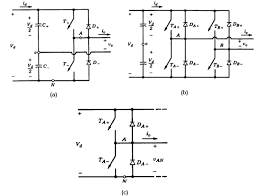
\includegraphics[scale=1.00]{images.png}
\caption{}
\label{}
\end{figure}




\section{convertidores CA-CD}

recodificador monofasico de media onda         

recodificador de onda completa con transformador con derivacion central

rectificador puente de onda completa
\begin{figure}[htp]
\centering
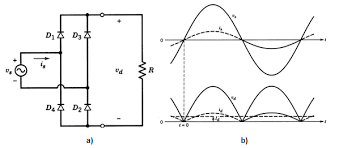
\includegraphics[scale=1.00]{descarga.png}
\caption{}
\label{}
\end{figure}

\url{http://catarina.udlap.mx/u_dl_a/tales/documentos/lem/moyaho_l_i/capitulo1.pdf}



\section{Convertidores CD-CD}
un convertidor elevador de voltaje de salida es mayor que el voltaje de entrada de ahi la palabra de elevador 
\begin{figure}[htp]
\centering
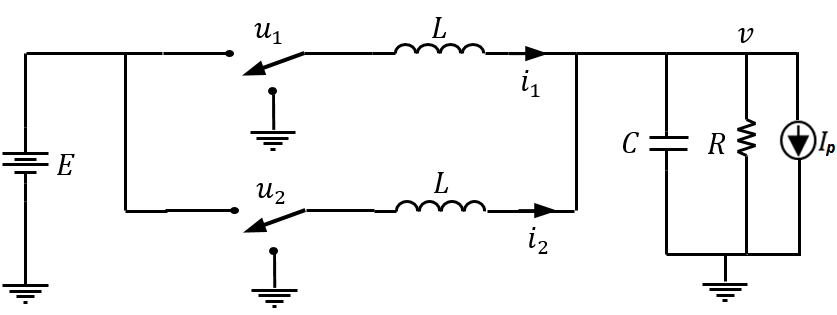
\includegraphics[scale=0.50]{Figura-1-Convertidor-CD-CD-Reductor-Paralelo.png}
\caption{}
\label{}
\end{figure}




 se llaman convertidor DC-DC a un dispositivo que convierte la corriente continua de una tension a otra. Suelen ser reguladores de conmutacion,dado a su salida una tension regulada y la mayor de las veces con limitacion de cotrriete 
 
 

 

\begin{figure}[htp]
\centering
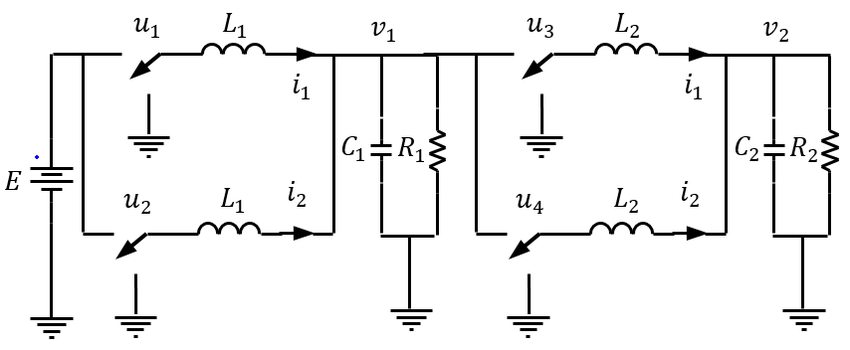
\includegraphics[scale=0.50]{Convertidor-cd-cd-reductor-paralelo-cascada.png}
\caption{}
\label{}
\end{figure}

\url{http:es.wikipedia.org/wiki/Convertidor_DC_a_DC}

\end{document}
